% ------------------------------------------------------------
\section{Calendar Week}
% ------------------------------------------------------------
% --------------------------------------------------- Slide --
\subsection{CW 32}
% ------------------------------------------------------------
\begin{frame}
  \frametitle{Review CW 32}
	\begin{itemize}
		\item More detailed FEA performed using remote access. Results and comparison with figures from Kitamura2004 are shown in next slides. - \textcolor{green}{Done}
		\item Acceptance letter for "Dissertations Anzeige" received from "Promotionsbuero". - \textcolor{green}{Done}
		\item Enrollment as promotion student as next step. \textcolor{yellow}{In Work}
	\end{itemize}
\end{frame}

\begin{frame}
  \frametitle{Review CW 32 - Model}
	\begin{figure}
		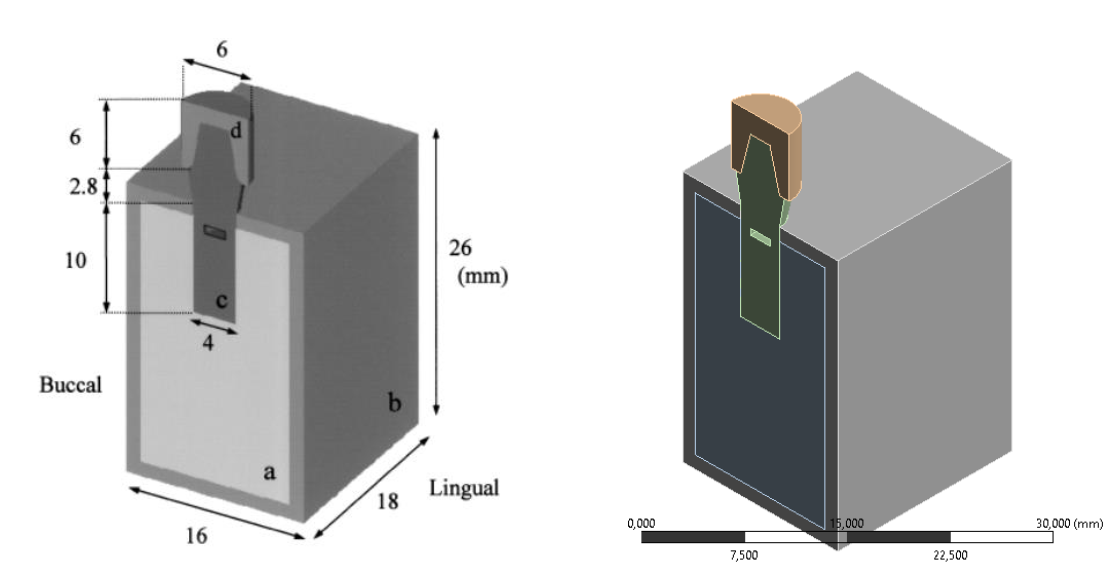
\includegraphics[width=0.8\textwidth]{pictures/CW32_1}
	\end{figure}
	\centering Kitamura2004 (Left) vs. Our work (right).
\end{frame}

\begin{frame}
  \frametitle{Review CW 32 - Bone Resorption}
	\begin{figure}
		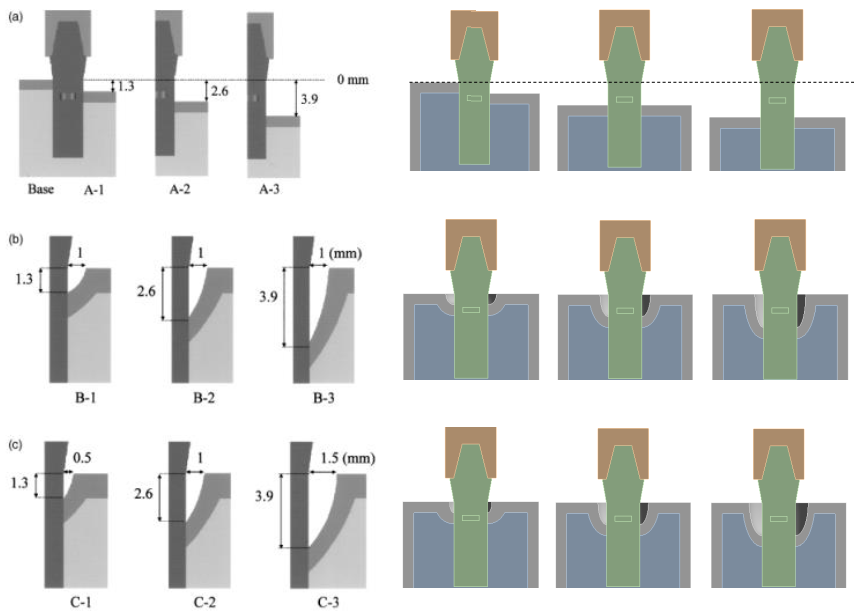
\includegraphics[width=0.7\textwidth]{pictures/CW32_2}
	\end{figure}
	\centering Various levels of bone resorption (Vertical and Conical). \\
	\centering Kitamura2004 (Left) vs. Our work (right).
\end{frame}

\begin{frame}
  \frametitle{Review CW 32 - Mesh}
	\begin{figure}
		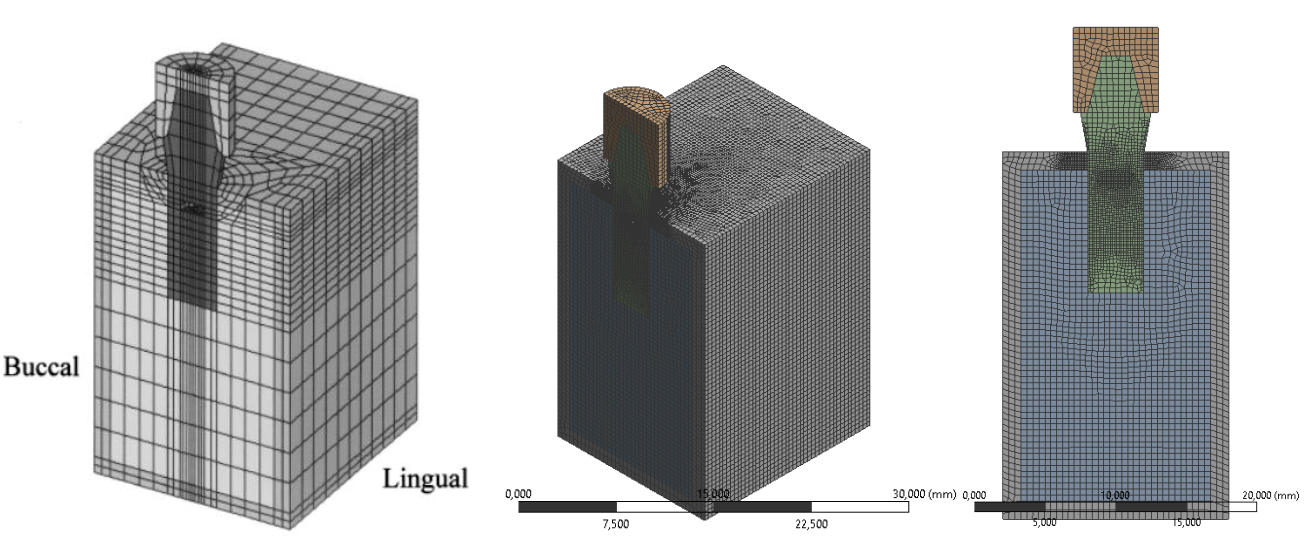
\includegraphics[width=0.8\textwidth]{pictures/CW32_3}
	\end{figure}
	\centering Mesh used for base model. \\
	\centering Kitamura2004 (Left) vs. Our work (right).
\end{frame}

\begin{frame}
  \frametitle{Review CW 32 - Cortical Bone - Equiv. Stress}
	\begin{figure}
		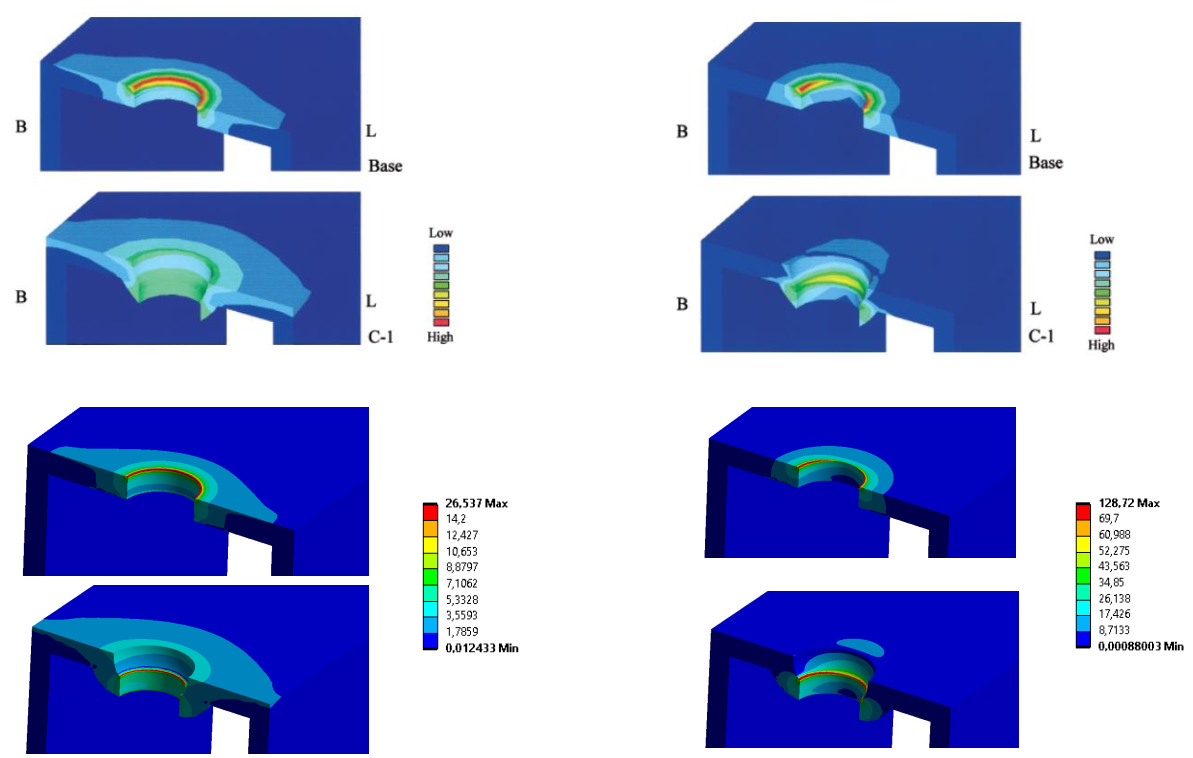
\includegraphics[width=0.8\textwidth]{pictures/CW32_4}
	\end{figure}
	\centering Base and C-1 model with axial (left) and lateral (right) loads. \\
	\centering Kitamura2004 (Top 2) vs. Our work (Bottom 2).
\end{frame}

\begin{frame}
  \frametitle{Review CW 32 - Cancellous Bone - Equiv. Stress}
	\begin{figure}
		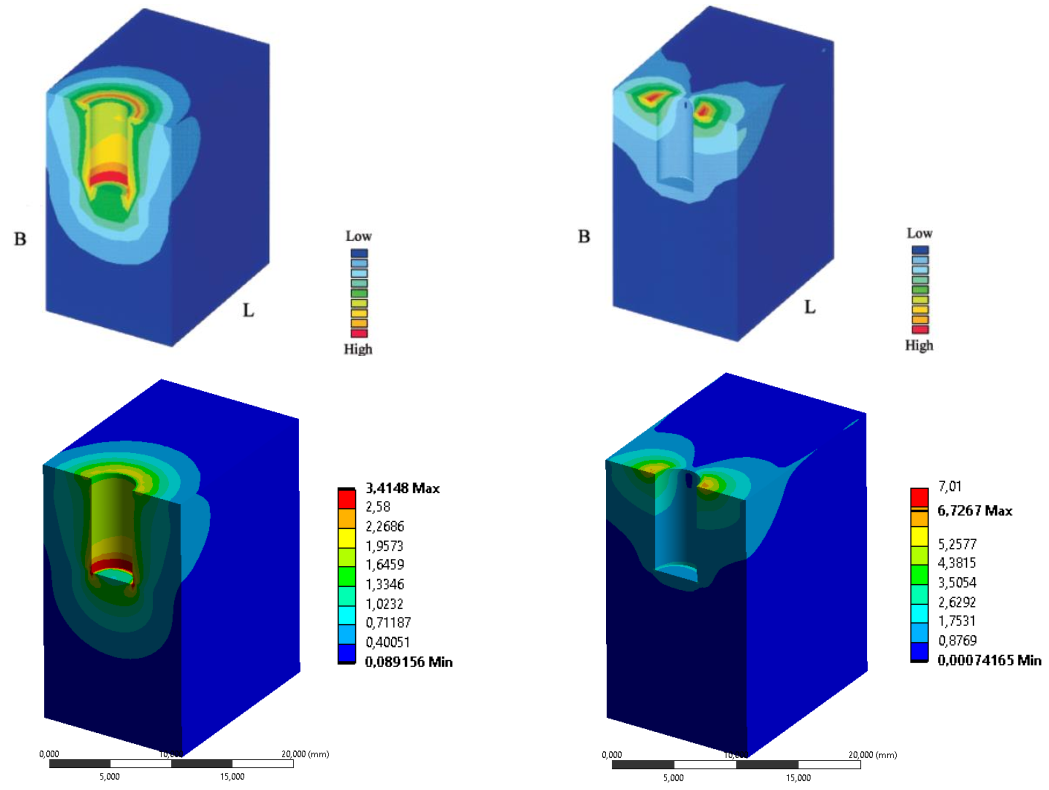
\includegraphics[width=0.6\textwidth]{pictures/CW32_5}
	\end{figure}
	\centering Base model with axial (left) and lateral (right) loads. \\
	\centering Kitamura2004 (Top) vs. Our work (Bottom).
\end{frame}

\begin{frame}
  \frametitle{Review CW 32 - Implant - Equiv. Stress}
	\begin{figure}
		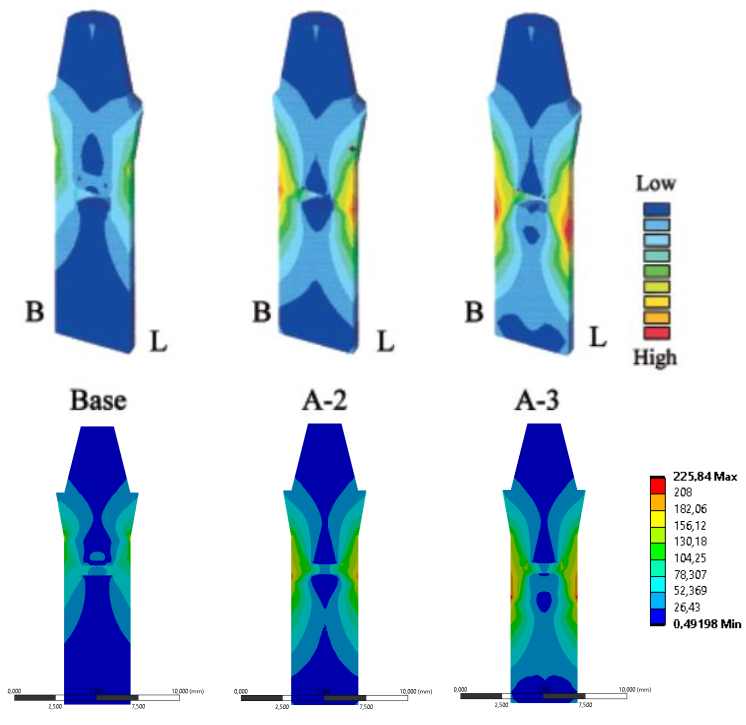
\includegraphics[width=0.5\textwidth]{pictures/CW32_6}
	\end{figure}
	\centering Base, A-2 and A-3 models with lateral loads. \\
	\centering Kitamura2004 (Top) vs. Our work (Bottom).
\end{frame}

% ------------------------------------------------------------
% --------------------------------------------------- Slide --
\subsection{CW 33}
% ------------------------------------------------------------
% ------------------------------------------------------------
\begin{frame}
  \frametitle{Outlook CW 33}
	\begin{itemize}
		\item Until now all geometries have been created manually. Initiate automation of geometry creation considering bone resorption. Note that only geometry will be automated, level of resorption still to be set manually.
	\end{itemize}
\end{frame}
% --------------------------------------------------- Slide --

